\documentclass[border=2pt]{standalone}
% Shared preamble for the standalone result plots (fig/src/*.tex).
% Compile:  tectonic -X compile fig/src/<name>.tex --outdir fig/src/out
% then copy fig/src/out/<name>.pdf over fig/<name>.pdf
%
% Palette matches the paper: wacvblue is main.tex's link colour, orange is xcolor's.
\usepackage{iftex}
\ifXeTeX
  \usepackage{fontspec}
  \setmainfont{texgyretermes}[Extension=.otf, UprightFont=*-regular,
    BoldFont=*-bold, ItalicFont=*-italic, BoldItalicFont=*-bolditalic]
\fi
\usepackage{pgfplots}
\pgfplotsset{compat=1.18}
\usepackage{amsmath}
\definecolor{wacvblue}{rgb}{0.21,0.49,0.74}
\pgfplotsset{
  resultaxis/.style={
    axis background/.style={fill=white},
    grid=major, ymajorgrids=true, xmajorgrids=false,
    grid style={gray!25, line width=0.3pt},
    tick align=outside, tick pos=left,
    label style={font=\small}, tick label style={font=\small},
    legend style={font=\small, draw=gray!50, fill=white, fill opacity=0.9,
                  text opacity=1, inner sep=2pt},
  },
  vidmark/.style={wacvblue, mark=*, thick, mark size=2.2pt},
  eegmark/.style={orange, mark=o, thick, dashed, mark size=2.2pt},
}

\begin{document}
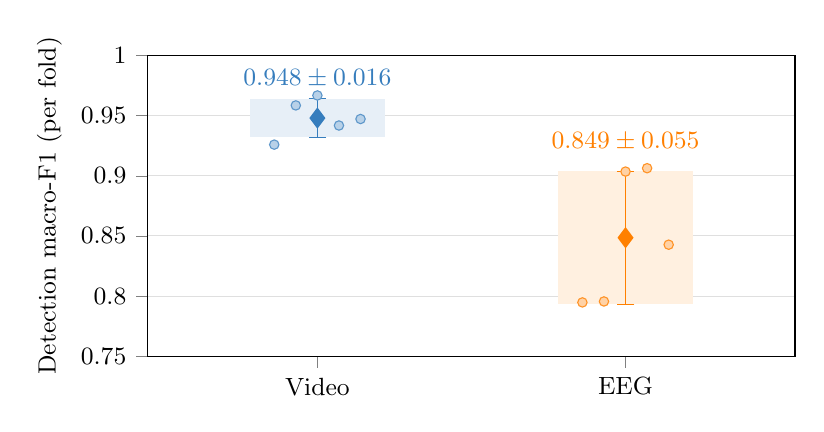
\begin{tikzpicture}
\begin{axis}[
  resultaxis,
  width=9.8cm, height=5.4cm,
  ylabel={Detection macro-F1 (per fold)},
  xtick={1,2}, xticklabels={Video, EEG},
  xmin=0.45, xmax=2.55, ymin=0.75, ymax=1.0,
  ytick={0.75,0.8,0.85,0.9,0.95,1.0},
  yticklabel style={/pgf/number format/fixed,/pgf/number format/precision=2},
]
% mean +/- sd bands
\fill[wacvblue!12] (axis cs:0.78,0.9320) rectangle (axis cs:1.22,0.9641);
\fill[orange!12]   (axis cs:1.78,0.7934) rectangle (axis cs:2.22,0.9037);
% per-fold points
\addplot[only marks, wacvblue!80, mark=*, mark size=1.7pt, fill=wacvblue!35]
  coordinates {(0.86,0.9259) (0.93,0.9585) (1.00,0.9668) (1.07,0.9418) (1.14,0.9472)};
\addplot[only marks, orange!85, mark=*, mark size=1.7pt, fill=orange!35]
  coordinates {(1.86,0.7947) (1.93,0.7955) (2.00,0.9035) (2.07,0.9063) (2.14,0.8427)};
% means with +/- sd error bars
\addplot[wacvblue, mark=diamond*, mark size=3.2pt, only marks, thick,
  error bars/.cd, y dir=both, y explicit] coordinates {(1.0,0.9480) +- (0,0.0161)};
\addplot[orange, mark=diamond*, mark size=3.2pt, only marks, thick,
  error bars/.cd, y dir=both, y explicit] coordinates {(2.0,0.8485) +- (0,0.0552)};
\node[wacvblue, font=\small, anchor=center] at (axis cs:1,0.981) {$0.948\pm0.016$};
\node[orange,   font=\small, anchor=center] at (axis cs:2,0.928) {$0.849\pm0.055$};
\end{axis}
\end{tikzpicture}
\end{document}
